	\newpage
\section{Ogólne określenie wymagań}		%1
%Ogólne określenie wymagań i zakresu programu (Czyli zleceniodawca określa wymagania programu) 




\subsection{Opis działania}  %1.1       

\hspace{0.60cm}Aplikacja na urządzenia mobilne umożliwiająca monitoring dokonań sportowych w dziedzinie biegania. Program ma umożliwić monitorowanie naszej aktywności biegowej. Aplikacja ma zapisywać przede wszystkim czas treningu, dystans, trasę uzyskaną dzięki modułowi GPS oraz intensywność treningu (np. wyliczając średnie tempo, średnią i maksymalną prędkość oraz skalone kalorie). Kożystając z aplikacji mamy mieć możliwość szczegółowej weryfikacji danych treningu, zarówno w trakcie jego trwania jak i po jego zakończeniu. Dodatkowo w podsumowaniu dzięki współpracy programu z GPS-em, można także spawdzić informacje o najniższym i najwyższym punkcie trasy. Szczegółowe statystyki mają pozwolić na analizę postępów i wyciągnięcie wniosków na przyszłość.

Treningi mają być zapisywane w pamięci. Użytkownik ma mieć możliwość zobaczenia statystyk wybranego treningu.

Aplikacja ma za zadanie także motywować nas do ćwiczeń, np. wysyłając nam powiadomienia, w ustalonym przez użytkownika momencie, o tym, że nie odbyliśmy jeszcze treningu.

Poza pomiarami w trakcie treningu, aplikacja ma także liczyć kroki, kiedy działa w tle.






\subsection{Opis wyglądu}  %1.2


\hspace{0.60cm}Na głównej stronie treningu, którą widzi użytkownik po otwarciu aplikacji, powinny znajdować się takie informacje jak:
\begin{itemize}
	\item Czas trwania aktywności,
	\item Prędkość w danym momencie,
	\item Średnia prędkość,
	\item Dystans,
	\item Spalone kalorie
\end{itemize}

Oprócz tego na stronie treningu Rys. \ref{rys:rysunek001} (s. \pageref{rys:rysunek001}) powinna znajdować się mapa, na której będzie pokazana aktualna pozycja uzytkownika oraz przebyta trasa.

Po zakończonym treningu aplikacja ma pokazać całą przebytą trasę na mapie oraz dać dostęp do szczegółowych statystyk treningu Rys. \ref{rys:rysunek002} (s. \pageref{rys:rysunek002}). Użytkownik ma mieć podgląd na wszystkie możliwe dane.

\begin{figure}[!htb]
	\centering
	\begin{minipage}{.5\textwidth}
		\centering
		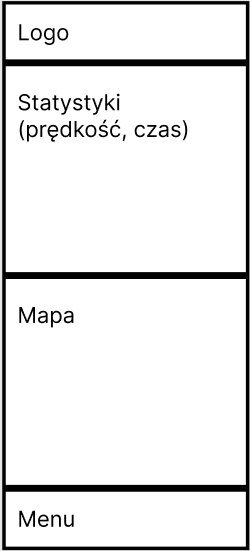
\includegraphics[width=.4\linewidth]{rys/ekran_treningu.png}
		\caption{Ekran treningu}
		\label{rys:rysunek001}
	\end{minipage}%
	\begin{minipage}{.5\textwidth}
		\centering
		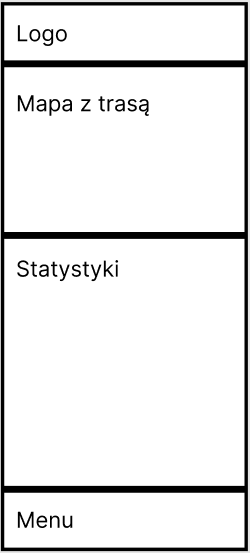
\includegraphics[width=.4\linewidth]{rys/ekran_podsumowania.png}
		\caption{Ekran podsumowania}
		\label{rys:rysunek002}
	\end{minipage}
\end{figure}

Ekran krokomierza Rys. \ref{rys:rysunek003} (s. \pageref{rys:rysunek003}) ma zawierać tylko liczbę zrobionych w~biezacym dniu kroków.

\begin{figure}[!htb]
	\centering
	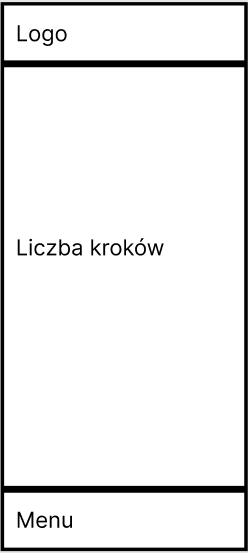
\includegraphics[width=.2\linewidth]{rys/ekran_krokomierza.png}
	\caption{Ekran krokomierza}
	\label{rys:rysunek003}
\end{figure}

Na dole aplikacji ma się znajdować menu za pomocą którego użytkownik może się przełączać pomiędzy ekranem krokomierza, treningu, odbytymi treningami i ustawieniami.

Ekran zawierający historię odbytych treningów powinien przedstawiać je w~postaci list. Ustawienia też powinny być przedstawione w postaci listy. 
 